\subsection{Electromagnetic Calorimeter} 
\label{sec:ecal}

The Ecal, depicted in Figure \ref{fig:ecal}, consists of $442$ lead-tungstate PbWO$_4$ crystals with avalanche photodiode (APD) 
readout and amplifiers. The short output pulse widths permit operation at very high rates. Indeed,(PbWO$_4$) crystals with APD readout 
are ideally suited to deal with the expected high radiation and high rate environment and they can operate in the fringe field of the HPS
magnetic field as well. The lead-tungstate modules, see Figure \ref{fig:module}, are taken from the Inner 
Calorimeter (IC) of the JLab CLAS detector, which was built by IPN Orsay (France) and other Hall B collaborators and was used
in a series of high energy electroproduction experiments. 
Orsay played a key role in the design and fabrication of the support frames, thermal enclosure, amplifiers,  
and motherboards of the IC, and is playing a similar role with the HPS ECal.  
The PbWO$_4$ crystals are $16$ cm long and tapered. The cross section of the front face is $1.3\times 1.3$ cm$^2$, 
and  $1.6\times 1.6$ cm$^2$ at the back. Modules in the ECal are arranged in two formations, as shown in Figure \ref{fig:ecal}. 
There are 5 layers in each formation; four layers have $46$ crystals and one has $37$. The ECal is mounted downstream of the 
analyzing dipole magnet at the distance of about $137$ cm from the upstream edge of the magnet. The two ECal modules are 
positioned just above and below the ECal vacuum chamber, through which the beam, radiated photons, and the wall of flame will pass
unimpeded. The innermost edge of the crystals is just $2$ cm from the beam. In order to stabilize the calorimeter's performance, 
the crystals, APDs, and amplifiers are enclosed within a temperature controlled environment, held constant at 
the level of 1\!\char23F. The energy resolution of the system, expected from operational experience with the IC, 
is $\sigma_E/E \sim 4.5\%/\sqrt{E}$ (GeV). As in the IC, PbWO$_4$ modules are connected to a motherboard that provides
power and transmits signals from individual APDs and amplifier boards to the data acquisition system. The ECal data is 
digitized using the JLAB FADC250, a 250 MHz flash ADC developed for the 12 GeV Upgrade. Pulse height information and spatial 
and timing information from each crystal are available for the trigger decision, which uses this information to reduce the trigger rate to a manageable $\sim 30$ kHz (see Section \ref{sec:triggerdaq} 
for details).

\begin{figure*}[t]
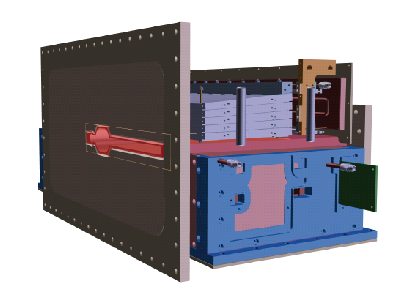
\includegraphics[width=\textwidth]{ecal/ECal.png}
\caption{\small{Arrangement of Ecal crystals. The two modules are positioned above and below the beam plane. Each module has 5 layers. 
There are 46 crystals in each layer, with the exception of the layers closest to the beam plane in which 9 crystals are removed to allow 
a larger opening for the outgoing electron and photon beams.}}\label{fig:ecal}
\end{figure*}

\begin{figure*}[t]
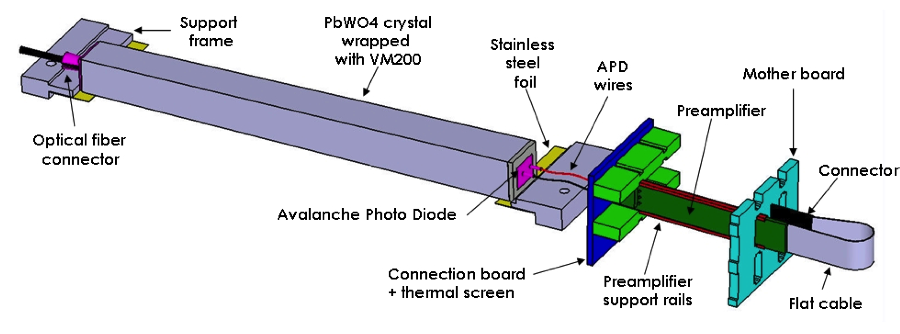
\includegraphics[width=\textwidth]{ecal/ecal_module.png}
\caption{\small{The ECal module is composed of a 16 cm long lead-tungstate crystal, Avalanche Photo Diode, and a amplifier 
board.}}\label{fig:module}
\end{figure*}

The HPS calorimeter described above was built and used during the HPS test run in April-May of 2012. This was the first time that 
a readout and trigger system utilizing the JLAB FADC250s had been used in a real experiment. The trigger algorithm was designed 
to satisfy the HPS 
event selection criteria and was implemented with newly developed FPGA-based trigger processors. Not all aspects 
of the trigger system were tested in the HPS Test Run because of the low interaction and background rates associated with photon running. But the 
ECal and its readout performed well and the critical goals for the Test Run run were 
achieved (see Section \ref{sec:testrun2012} for details). While the ECal performance during the test run was satisfactory, several aspects are in need of improvement, as described below.   

\subsubsection{Improvements to the existing calorimeter}

There are no plans for major mechanical changes to the ECal proper. The crystals, support frames, and thermal enclosure operated as designed and will stay unchanged. Most of the needed changes are related to the signal readout chain and problems encountered in the Test Run with the ECal and FADC250. Plans for  
modifications and/or improvements are as follows: 

\begin{enumerate}
\item {\bf Replacing the ECal mounting system} - 
During the test run the ECal was supported by the Hall-B pair spectrometer mount rails which also support the pair spectrometer hodoscopes. 
Photon running prevented the installation of the ECal vacuum chamber and relaxed the requirements for precise ECal alignment. Consequently, the ECal was simply hung from the mount rails using  long threaded rods. This system must be replaced with a more robust and finely adjustable (both horizontally and vertically) support mechanism to  align the  ECal correctly with the ECal vacuum chamber.

\item {\bf Modification of motherboards} - One of the issues  faced during the test run was excess noise on some channels of the motherboards. 
Most missing channels, those which are absent on the performance figures in Section \ref{sec:testrun2012}, were in fact switched off because they were very noisy and there was no time to debug them. New motherboards will be designed and built to resolve these noise issues. One of options under discussion is to replace long motherboards with shorter ones with power and signal connectors 
located on the top (for the top module) and the bottom (for the bottom module) of the thermal enclosure. 

\item {\bf Signal splitting} - From the experience gained with the JLAB FADC250 by the HPS group and others, it is evident that the FADCs can be used both for precision time measurements and as 
real-time scalers simply by developing the appropriate firmware.
Precise pulse timing will allow tighter coincidence windows and lower backgrounds, and real time scalers will provide good online monitoring of detector performance. The present ECal readout configuration uses signal splitters to divide the preamplifier signal in  a 2:1 ratio, sending 
$2/3$ of the signal to a discriminator that has built-in scalers and feeds the TDC channel. The other $1/3$ of the 
signal goes to the FADC for the energy measurement. Removing the splitter will increase the signal on the FADC input by $\times 3$. This will allow use of a new lower gain amplifiers with much improved noise level. This effort will make use of newly developed readout system for the CLAS12 Forward Tagger calorimeter. This development is joined venture of IPN Orsay and INFN Genova groups who are also in the HPS collaboration.

 
\item {\bf New preamplifiers} - A low noise, low gain preamplifiers will be needed to take advantage of increased signal on the input of FADC after removing the spliter. The impact of the lower noise/threshold system is twofold: first it 
will improve the ECal's energy resolution; and second it will make the ECal sensitive to minimum ionizing particles which pass through the crystals transversely. With sensitivity to cosmic ray muons, which will pass through the ECal transversely when it is installed in HPS, the Ecal crystals can be calibrated for MIPS, and their effective gains balanced.  HPS collaborators from INFN Genova have shown that with such a low noise, low threshold system, the ECal can distinguish the MIP energy deposition from noise, see Figure \ref{fig:mip5x5}.


\end{enumerate}

\begin{figure*}[t]
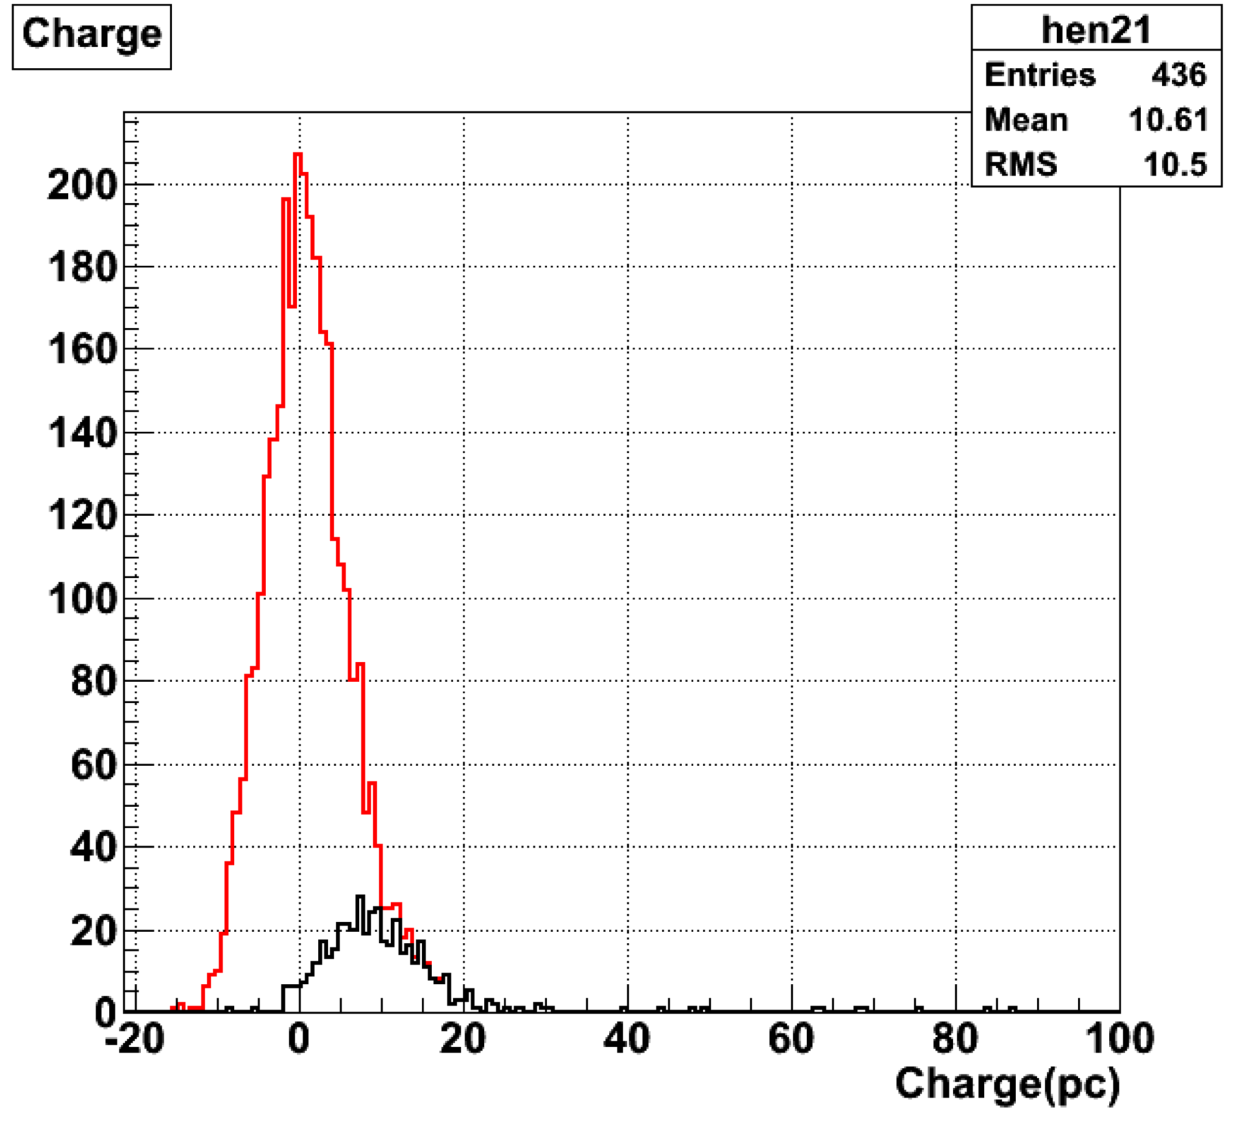
\includegraphics[scale=0.4]{ecal/MIP_5x5_APD.png}
\caption{\small{Charge distribution from readout of the HPS calorimeter crystal with Hamamatsu S8664-55 APD, and the new low noise amplifier board. The red line histogram corresponds to the charge distribution for all triggers coming from the scintillators positioned above and below the crystal. The black line shows the distribution for hits in the crystal 
within $100$ ns of the trigger signal. }}\label{fig:mip5x5}
\end{figure*}

